\chapter{Foundations}

This chapter provides information on overarching as well as foundational concepts relevant to the following chapters. Specifically, we cover two areas.

\begin{enumerate}
    \item \textbf{Scholarly Data}\\
        First, we give an overview of the academic publication ecosystem and its relation to the landscape of scholarly data. Understanding the parts involved and relations between them is helpful for understanding decisions made in the system design and method development of the approaches presented later on.
    \item \textbf{Data Mining \& Information Extraction}\\
        Second, we present relevant evaluation metrics from the areas of data mining and information extraction. These are essential for understanding the research goals as well as the results that were achieved.
\end{enumerate}

\section{Scholarly Data}

% What do I want to say and convey here?
% - 

\begin{figure}[bt]
  \centering
  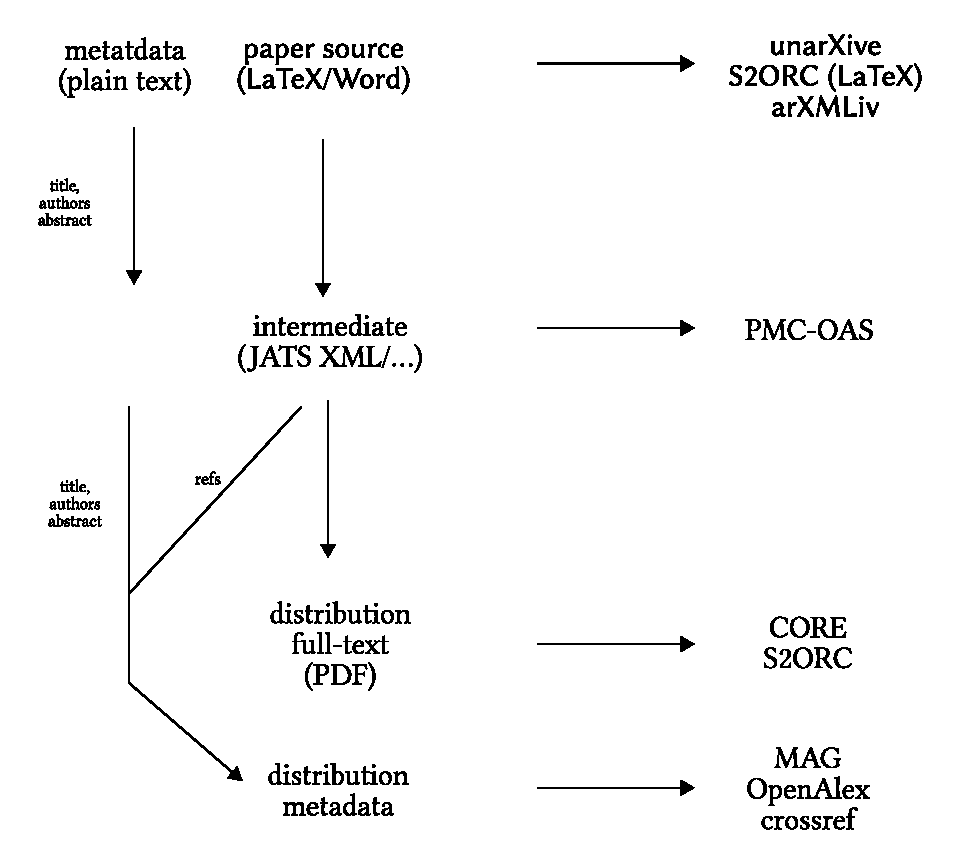
\includegraphics[width=0.7\linewidth]{figures/foundations/scholarly_data_lifecycle_dummy}
  \caption[Scholarly data lifecycle]{Scholarly data lifecycle}
  \label{fig:foundations-datalifecycle}
\end{figure}

in Figure~\ref{fig:foundations-datalifecycle}

Joanne Cohn sending around e-prints~\cite{Feder2021,Turner2012}

June 1991 meets Paul Ginsparg who then goes on to start arXiv~\cite{Ginsparg2011a,Ginsparg2011}

arXiv used 1998 for scholarly IE~\cite{Nanba1998}

metadata dump since 2020(?) available on Kaggle~\cite{arxiv_kaggle_dataset}

\subsection{\LaTeX}

\subsection{Further Data Formats}

\paragraph{Word}

\paragraph{JATS XML}

\paragraph{PDF}

\paragraph{Triple Formats}
RDF, Turtle, JSON-LD, ... (relevant for metadata)

% document classes and packages provide semantic macros and translate them
% into visual output, but user can at any time also use visual primitives
% directly


\section{Data Mining \& Information Extraction}

% What do I want to say and convey here?
% - 

\subsection{Data Quality Metrics}

\subsection{Model Evaluation Metrics}
